% !TEX TS-program = XeLaTeX
% !TEX spellcheck = en-US
\documentclass[aspectratio=169]{beamer}

\usetheme{bi}

\title{Lecture 5:\\ Model selection, evaluation and assessment}
\institute{GRA4160: Predictive modelling with machine learning}
\date{February 8th 2023}
\author{Vegard H\o ghaug Larsen}

\begin{document}

\maketitle

\frame{
	\frametitle{Plan for today:}
	\begin{enumerate}
		\item Model selection, evaluation and assessment
		\item Information criteria
		\item Cross-validation
		\item Bias-variance trade-off
	\end{enumerate}
}

\frame{
	\frametitle{}
	\begin{center}
		\Huge{Model selection}
	\end{center}
}

\frame{
	\frametitle{Model Selection}
	\begin{itemize}
		\item Model selection is the process of choosing the best model from a set of candidate models
		      \pause
		\item The simplest approach is to compare the performance of different models on a held-out test set, and choose the model with the best performance
		      the    \pause
		\item This approach can lead to overfitting, where the model that performs best on the validation set is not the best model for the problem in general
		      \pause
		\item \textbf{Cross-validation} is a more robust approach where we select the model that performs best on the validation set in each fold of the data
		      \pause
		\item Another alternative is to use \textbf{inforation criteria} where we e.g., can calculate the AIC or BIC value for each candidate model, and choose the model with the lowest value
	\end{itemize}
}

\frame{
	\frametitle{}
	\begin{center}
		\Huge{Model Evaluation}
	\end{center}
}

\frame{
	\frametitle{Model Evaluation}
	\begin{itemize}
		\item Model evaluation is the process of evaluating the performance of a model on new unseen data
		      \pause
		\item This is typically done by dividing the data into training and testing sets, or by using cross-validation techniques
		      \pause
		\item The goal of model evaluation is to determine how well the model is likely to perform in practice
		      \pause
		\item Common metrics used for model evaluation include accuracy, precision, recall, ROC curve, and AUC
		      \pause
		\item Visualizations such as confusion matrices and decision boundaries can also be useful for evaluating the performance of a model
	\end{itemize}
}

\frame{
	\frametitle{Metrics used for model evaluation}
	\begin{itemize}
		\item \textbf{Accuracy} is the fraction of predictions that are correct, including both true positives and true negatives.
		      \pause
		\item \textbf{Precision} is the fraction of positive predictions that are correct. Precision is particularly important in scenarios where false positives are more costly
		      \pause
		\item \textbf{Recall} measures the ability of a model to correctly identify all positive instances in a dataset. Recall is crucial when false negatives are more critical
		      \pause
		\item \textbf{ROC} curve is a plot of the true positive rate against the false positive rate. It shows the performance of a classification model at all classification thresholds
		      \pause
		\item \textbf{AUC} is the area under the ROC curve. Provides an aggregate measure of performance across all possible classification thresholds
	\end{itemize}
	More details: See exercise 5 in the exercise notebook
}

\frame{
	\frametitle{Understanding the Confusion Matrix}
	\begin{itemize}
		\item A \textbf{Confusion Matrix} is a table used to describe the performance of a classification model.
		      \pause
		\item It contains four components:
		      \begin{itemize}
			      \item \textbf{True Positives (TP)}: Correctly predicted positive instances
			      \item \textbf{True Negatives (TN)}: Correctly predicted negative instances
			      \item \textbf{False Positives (FP)}: Incorrectly predicted positive instances (Type I error)
			      \item \textbf{False Negatives (FN)}: Incorrectly predicted negative instances (Type II error)
		      \end{itemize}
		      \pause
		\item The matrix helps in calculating various performance metrics:
		      \begin{itemize}
			      \item Precision = TP / (TP + FP)
			      \item Recall = TP / (TP + FN)
			      \item Accuracy = (TP + TN) / (TP + TN + FP + FN)
		      \end{itemize}
		      \pause
		\item It provides a holistic view of the model's performance, beyond just accuracy.
	\end{itemize}
}


\frame{
	\frametitle{}
	\begin{center}
		\Huge{Model Assessment}
	\end{center}
}

\frame{
	\frametitle{Model Assessment}
	\begin{itemize}
		\item Model assessment is a broad concept that covers the evaluation of multiple aspects of a trained model.
		      \pause
		\item It involves evaluating the model's performance on new data and assessing factors like:
		      \begin{itemize}
			      \item \textbf{Complexity}: How intricate is the model? (e.g., number of parameters)
			      \item \textbf{Interpretability}: How easily can we understand the model’s decisions?
			      \item \textbf{Computational Efficiency}: How much computational resources does it require?
			      \item \textbf{Scalability}: Can it handle increasing data or complexity?
		      \end{itemize}
		      \pause
		\item Includes conducting sensitivity analyses or stress tests to determine the model's performance under varying conditions or scenarios, ensuring robustness and reliability.
		      \pause
		\item Emphasizes the importance of techniques like cross-validation to ensure generalizability to new data.
	\end{itemize}
}

\frame{
	\frametitle{}
	\begin{center}
		\Huge{Information criteria}
	\end{center}
}

\frame{
	\frametitle{Introduction to Information Criteria}

	\begin{itemize}
		\item Information Criteria are statistical tools used to compare and select models.
		      \pause
		\item They help in balancing model fit (how well a model describes the data) against model complexity (number of parameters).
		      \pause
		\item The goal is to find a model that adequately explains the data but is not overly complex.
		      \pause
		\item Commonly used Information Criteria include Akaike Information Criterion (AIC) and Bayesian Information Criterion (BIC).
		      \pause
		\item These criteria are based on principles from information theory and statistical likelihood.
	\end{itemize}
}

\frame{
	\frametitle{Akaike Information Criterion (AIC) and Bayesian Information Criterion (BIC)}

	\begin{itemize}
		\item \textbf{Akaike Information Criterion (AIC)}:
		      \begin{itemize}
			      \item Focuses on the trade-off between the goodness of fit and model complexity.
			      \item Lower AIC values indicate a better model.
			      \item Calculated as: $AIC = 2k - 2ln(L)$, where $k$ is the number of parameters, and $L$ is the likelihood of the model.
		      \end{itemize}
		      \pause
		\item \textbf{Bayesian Information Criterion (BIC)}:
		      \begin{itemize}
			      \item Similar to AIC but includes a stronger penalty for models with more parameters.
			      \item Favors simpler models more than AIC.
			      \item Calculated as: $BIC = ln(n)k - 2ln(L)$, where $n$ is the sample size.
		      \end{itemize}
		      \pause
		\item Both AIC and BIC are used for model selection, but they have different approaches and interpretations.
	\end{itemize}
}

\frame{
	\frametitle{}
	\begin{center}
		\Huge{Cross validation}
	\end{center}
}

\frame{
	\frametitle{$k$-fold cross-validation}
	\begin{itemize}
		\item The original dataset is randomly partitioned into $k$ equal-sized subsets, or folds.
		      \pause
		\item In each iteration, one fold is used as the test set and the remaining $k-1$ folds are used as the training set.
		      \pause
		\item This process is repeated $k$ times, with each of the $k$ folds used exactly once as the test set.
		      \pause
		\item Provides a more reliable estimate of the model's performance by using all the data for both training and testing, reducing both bias and variance.
		      \pause
		\item Particularly useful when the amount of data available is limited.
	\end{itemize}

	\pause

	Common values of $k$ are 5 or 10. The choice of $k$ depends on the dataset size and computational resources. Larger $k$ values yield more reliable performance estimates but increase computational cost and may have higher variance in test performance.
}

\frame{
	\frametitle{}
	\begin{center}
		\Huge{The Bias-Variance trade-off}
	\end{center}
}

\frame{
	\frametitle{The Bias-Variance Trade-off}
	\begin{itemize}
		\item A fundamental concept in machine learning that relates to the performance of a model on new data.
		      \pause
		\item Bias refers to the error due to overly simplistic assumptions in the learning algorithm, leading to systematic deviation from the true values (underfitting)
		      \pause
		\item Variance refers to the error due to too much complexity in the learning algorithm, causing sensitivity to fluctuations in the training data (overfitting).
		      \pause
		\item High bias can result in a model that misses relevant relations between features and target outputs (underfitting).
		      \pause
		\item High variance can cause the model to model the random noise in the training data, rather than the intended outputs (overfitting).
		      \pause
		\item The goal is to achieve a balance between bias and variance, leading to a model that generalizes well to new data. This often involves model tuning and selection of appropriate algorithms.
	\end{itemize}
}

\frame{
	\frametitle{High bias and high-variance}
	\begin{itemize}
		\item High variance refers to a model that overfits the training data
		\item High variance can be addressed by simplifying the model or by adding regularization techniques
		      \pause
		\item High bias refers to a model that underfits the training data
		\item High bias can be addressed by using a more complex model, increasing the number of features, or reducing regularization
	\end{itemize}
}

\frame{
	\frametitle{Example of high bias}
	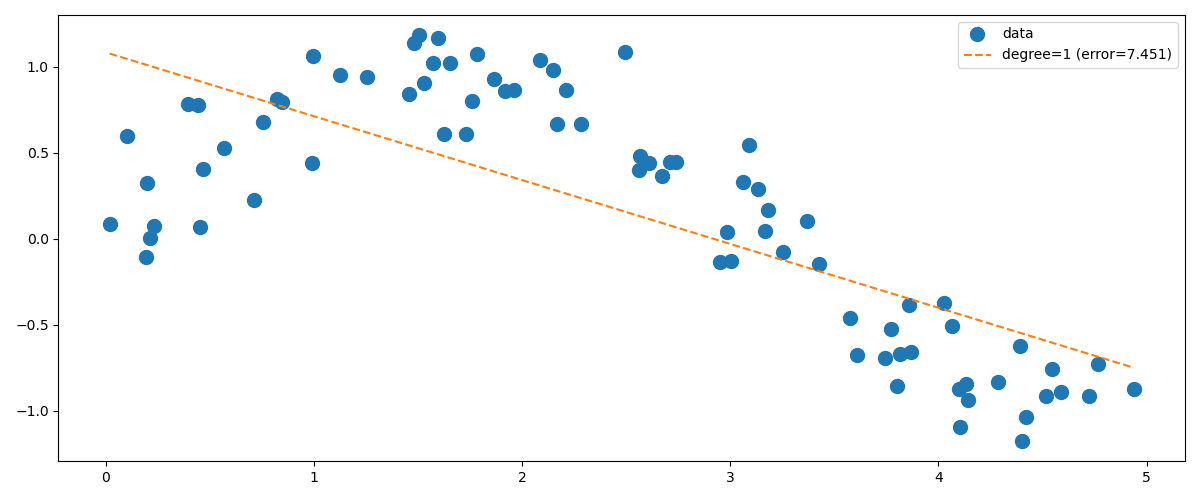
\includegraphics[scale=0.5]{figures/bias_variance_tradeoff_1.png}
}

\frame{
	\frametitle{Example of high variance}
	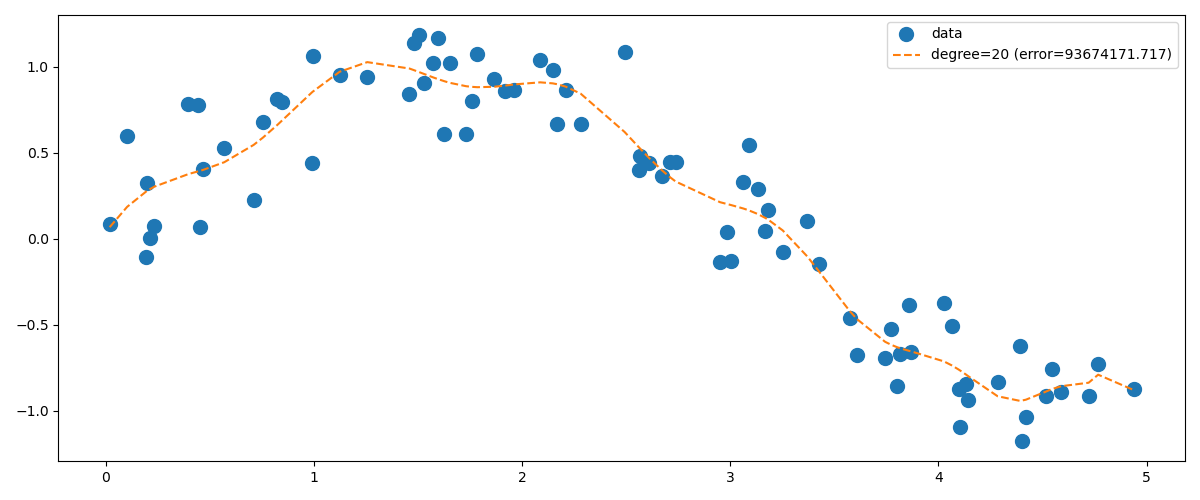
\includegraphics[scale=0.5]{figures/bias_variance_tradeoff_2.png}
}

%\frame{
%	\frametitle{Exercise: Model selection, assessment and evaluation}
%	\begin{itemize}
%		\item Use cross-validation to evaluate the performance of a $k$-nearest neighbors (KNN) model trained on the iris dataset. Vary the number of neighbors and compare the resulting cross-validation scores. Which value of $k$ gives the best performance?
%		\item Train different models on the iris dataset and compare their performance using accuracy and a confusion matrix. Which model performs best?
%		\item Perform $k$-fold cross-validation on the iris data and compare the performance of several models such as KNN, decision trees, and logistic regression. Which model performs best?
%		\item Train a decision tree on the iris dataset. Use \texttt{GridSearchCV} to find the best hyperparameters for \texttt{max\_depth}, \texttt{min\_samples\_leaf}, and \texttt{min\_samples\_split}. What is the model accuracy with optimized hyperparameters?
%	\end{itemize}
%}

\end{document}